Les automates à files définis à la section \ref{fifo} sont plus puissants que les ADF définis dans la section \ref{adf}. En effet, les systèmes de transitions associés ont potentiellement une infinité de configurations. Dans ces conditions, il n'est pas possible de faire une exploration exhaustive des états pour trouver lesquels sont acceptants.

À la place, une propriété dite de sécurité est définie. Si un état respecte cette propriété, il est \emph{sûr}. Si il y a moyen de prouver que la totalité des états de l'automate respectent cette propriété, l'automate est considéré comme sûr. Si au contraire, un exemple de violation de la propriété est trouvé, l'automate peut être déclaré comme à risque.

L'idée dès lors est de travailler non pas avec un système de transitions infini mais avec une représentation construite pour être finie dans un vaste ensemble de problèmes. Cette représentation est le langage de trace défini dans la section \ref{trace}.

En supposant que celui-ci est régulier, il est possible d'utiliser l'algorithme d'Angluin de la section \ref{angluin} pour l'apprendre. Cependant, ce langage n'est qu'un concept et le professeur n'a accès qu'à un automate à files $F$. Pour cette raison, les oracles d'appartenance et d'équivalence sont adaptés pour répondre à une requête entre un langage fourni par l'élève et $F$.

La figure \ref{fig:lever} donne une vue schématique de ce nouvel algorithme d'Angluin modifié.


\begin{figure}[H]
	\centering

	\resizebox{\textwidth}{!}{
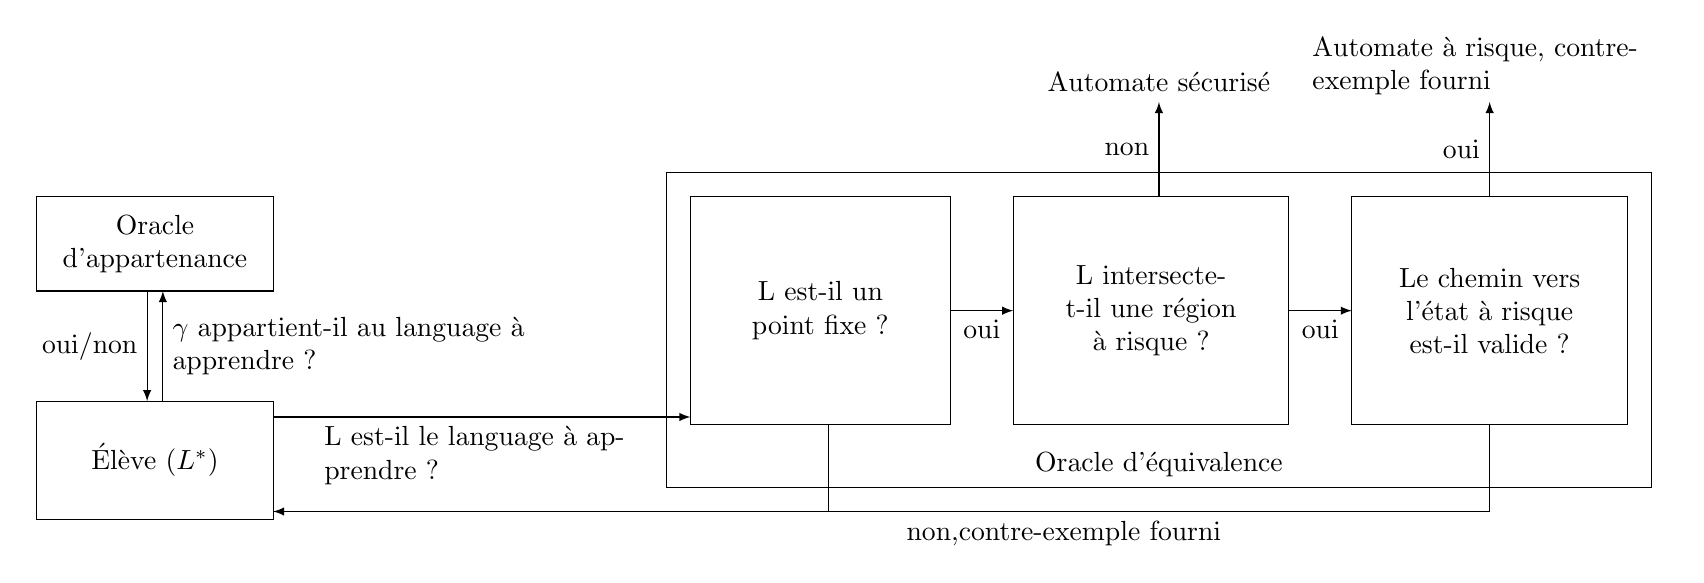
\begin{tikzpicture}
	\tikzset{>=latex}

  \draw (-3,-2.9) rectangle (0,-4.4) node[pos=.5] {Élève ($L^*$)};
  \draw (5,0) rectangle (17.5,-4);
	\draw[->] (0,-3.1) -- (5.3,-3.1) node[pos=0.5,below,text width=4cm] {L est-il le language à apprendre ?};

  \draw (-3,-0.3) rectangle (0,-1.5) node[pos=.5,text width=3cm,align=center] {Oracle\\ d'appartenance};
  \draw[->] (-1.4,-2.9) -- (-1.4,-1.5) node[pos=0.5,right,text width=5cm] {$\gamma$ appartient-il au language à apprendre ?};
  \draw[<-] (-1.6,-2.9) -- (-1.6,-1.5) node[pos=0.5,left] {oui/non};

  \node[draw=none] at (11.25, -3.7) {Oracle d'équivalence};

  \draw (5.3, -0.3) rectangle (8.6, -3.2) node[pos=0.5,text width=3cm,align=center] {L est-il un point fixe ?};
  \draw (9.4, -0.3) rectangle (12.9, -3.2) node[pos=0.5,text width=3cm,align=center] {L intersecte-t-il une région à risque ?};
  \draw (13.7, -0.3) rectangle (17.2, -3.2) node[pos=0.5,text width=3cm,align=center] {Le chemin vers l'état à risque est-il valide ?};

  \draw[->] (8.6, -1.75) -- (9.4,-1.75) node[pos=0.5,below] {oui};
  \draw[->] (12.9, -1.75) -- (13.7,-1.75) node[pos=0.5,below] {oui};
  \draw[->] (15.45, -4.3) -- (0, -4.3) node[pos=0.35,below] {non,contre-exemple fourni};
  \draw[-] (7.05, -3.2) -- (7.05, -4.3);
  \draw[-] (15.45, -3.2) -- (15.45, -4.3);

	\draw[->] (11.25,-0.3) -- (11.25,0.9)node[pos=0.5,left] {non};
	\draw[->] (15.45,-0.3) -- (15.45,0.9)node[pos=0.5,left] {oui};

	\node[draw=none] at (11.25, 1.15) {Automate sécurisé};
	\node[draw=none,text width=4.5cm] at (15.45, 1.36) {Automate à risque, contre-exemple fourni};


\end{tikzpicture}
}
\caption{Vue schématique de l'algorithme d'Angluin pour LeVer\cite{Vardhan04}}\label{fig:lever}
\end{figure}


\emph{LeVer} est le nom de cette technique. En particulier, on peut noter sur ce schéma que l'oracle d'équivalence peut non seulement répondre oui ou non mais également interrompre l'apprentissage s'il est possible de se prononcer sur la sûreté d'un automate à files $F$. Pour rappel, $L(F)$ n'est pas régulier en général. Pouvoir se prononcer sur la sûreté de $F$ étant possible, il n'est ni utile ni forcémment possible de continuer à appliquer $L^*$ pour obtenir une meilleure approximation $L$ du langage de trace de $F$. 
